\chapter{Architecture du backend}

\section{Entités}
\begin{figure}[h]
  \center
  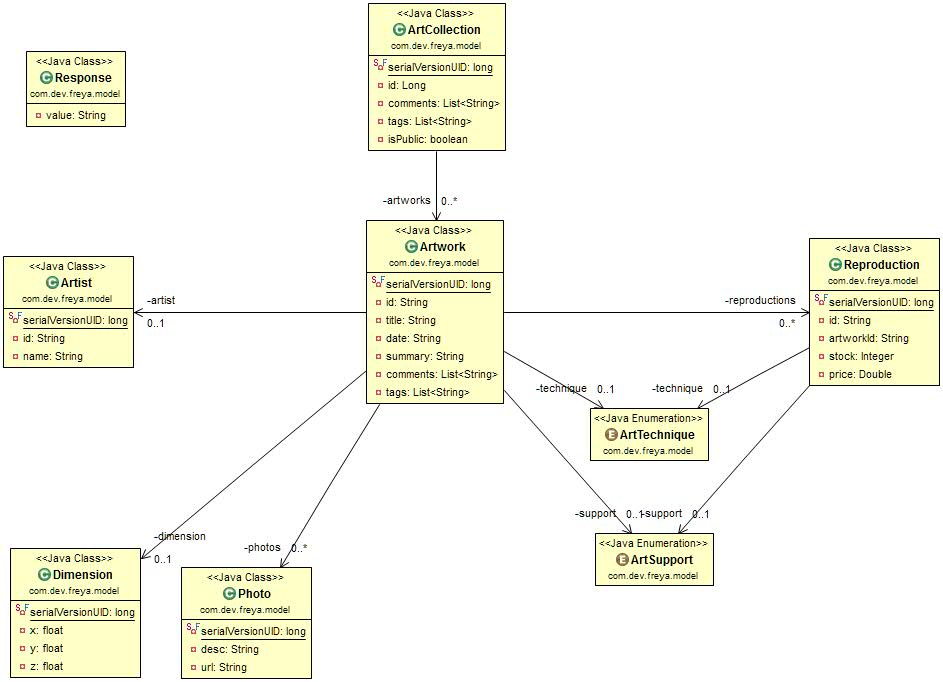
\includegraphics[width=1.0\textwidth]{resources/model_diagram.jpg}
  \caption{Diagramme de classe des entités}
  \label{fig:model_diagram}
\end{figure}

\newpage
\section{Conception}
Une des difficultés majeures de ce projet a été de concevoir correctement les
relations entre les entités afin d’être en accord avec les restrictions de GAE.
Étant donné que le \emph{datastore} est une base de données NoSQL, il fallait
respecter plusieurs contraintes supplémentaires.\\

Une des contraintes est qu’il faut qu’une entité fille encode la clé de son
parent dans sa propre clé. Cela signifie que quand une entité fille est
persistée, son parent ne peut plus changer (c.à.d être remplacé par un autre
parent). Ceci est dû au fait que les entités fille et parent sont placées dans
le même \emph{entity group}, et qu’une entité ne peut appartenir qu’à un seul
\emph{entity group}.\\

Pour des raisons de performance, le \emph{datastore} met en place d’autres
restrictions au niveau des requêtes. En effet, certaines opérations ne sont pas permises
(subqueries, fonction size, joins complexes, opérateur MEMBER OF sur une
collection non-primitive, et d'autres).\\

Pour gérer les paramètres optionnels pour filtrer les recherches, nous avons
utilisé l’API Criteria\footnote{JPA Criteria API:
\url{http://www.objectdb.com/java/jpa/query/criteria}} de JPA afin d’avoir un
code propre et maintenable, et qui est beaucoup plus robuste comparé à la
création de la requête par concaténation de chaînes.\\

Afin d'améliorer les performances du backend, nous avons aussi mis en place
Memcache\footnote{Memcache:
\url{https://developers.google.com/appengine/docs/java/memcache/}}, un système
de cache afin d'accélérer les requêtes d'écriture.
